%%%%%%%%%%%%%%%%%%%%%%%%%%%%%%%%%%%%%%%%%%%%%%%%%%%%%%%%%%%%%%%%%%%%%%%%%%%
\section{Processors for Embedded Systems}
%%%%%%%%%%%%%%%%%%%%%%%%%%%%%%%%%%%%%%%%%%%%%%%%%%%%%%%%%%%%%%%%%%%%%%%%%%%
\nsl{Embedded systems need special processors. A standard PC processor isn't suitable, as the microprocessor used doesn't operate independently. It has to be implanted on a motherboard, which serves as the communication interface between the processor and other input/output devices. This involves increased costs and such a system occupies a large space.
\newline
Shifting our focus to microcontrollers, we observe that an 8-bit microcontroller possesses small computing power and has too many restrictions in building an appropriate internal or external memory. So these types of processors are also not suitable for a sophisticated embedded system. The above mentioned restrictions are not evident when working with 16- and 32-bit microcontrollers. A big advantage of these types of microcontrollers is that nearly every type of interface is available which we might have to use in an embedded system.
\newline
If an Embedded application/project allows us to use a small motherboard (no hard discs and usually no GUI 'graphical user interfaces' etc.) then it makes sense to deploy an ``Embedded PC'' or a PC/104 system. Such systems contain a special, so called ``Mobile microprocessor'' like ``Pentium M'' or ``Geode'' or ``XScale''. These processors are variants of standard 8086-type microprocessors (Pentium M and Geode). If we are working with these Embedded PC's, then you have access to support in the form of well known standard PC tools like compilers, linkers and operating systems. 
\newline
Another type of processor which could be present in an embedded system is a signal processor. A signal processor has much more computing power than a microcontroller. But on the contrary to a microprocessor, a signal processor has nearly the same interfaces available in a microcontroller. The disadvantage of using a signal processor is that there aren't much development tools available.
}

\begin{description}
\bigskip
\item[{\rot\bf Microprocessors for Embedded Systems }]~\\[-3ex]
\bi
	\ite use a special version of an 8086-type of microprocessors (Pentium M or Geode)
	\ite these microprocessor are integrated in an ``embedded PC'' or a ``PC/104-system''
	\ite these type of PCs' work without any hard disc (and without any cooling system)
	\ite instead of a hard disc, a ``FLASH Memory'' is used (e.g. SD-Card)
	\ite if a graphical user interface is available, then the ``graphical processing unit'' is a part of the microprocessor.
\ei
\os{\newpage}
\begin{figure}[!hbtp]
     \begin{center}
	  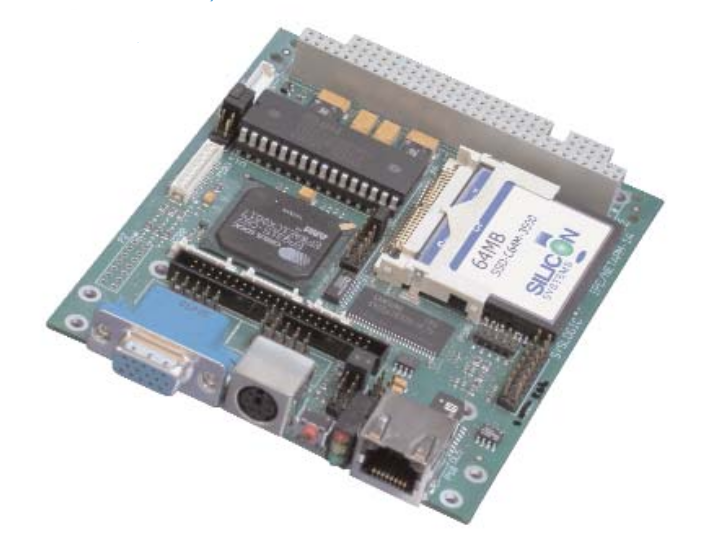
\epsfig{file=figures/Fig_3_1_SBC,width=0.7\textwidth}\\
	  \caption{Embedded PC as Single Board Computer}
     \end{center}
\end{figure}
\os{\newpage}     

\begin{figure}[!hbtp]
     \begin{center}
	  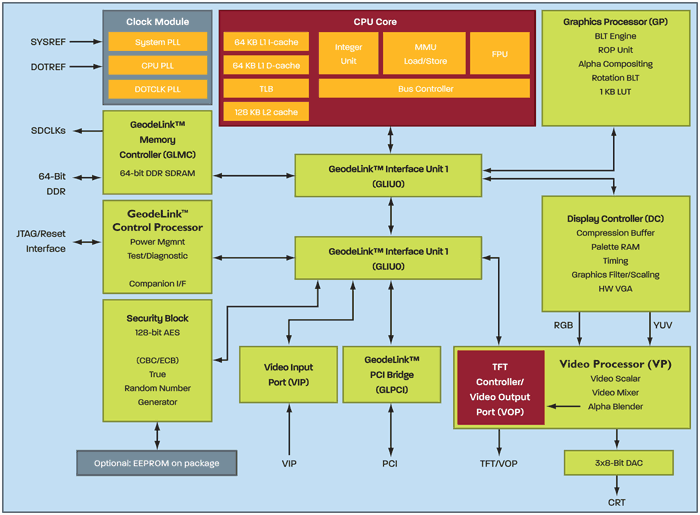
\epsfig{file=figures/Fig_3_2_Blockdiagram_Geode,width=0.8\textwidth}\\
	  \caption{Blockdiagram of a Geode-Microprocessor}
     \end{center}
\end{figure}
\os{\newpage}    

\begin{figure}[!hbtp]
     \begin{center}
	  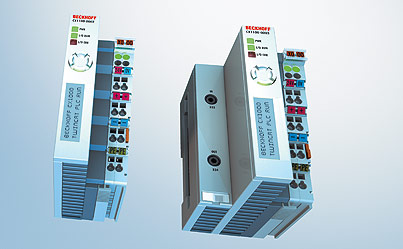
\epsfig{file=figures/Fig_3_3_Embedded_PC,width=0.9\textwidth}\\
	  \caption{A different type of Embedded PC}
     \end{center}
\end{figure} 
\os{\newpage}

\item[{\rot\bf Signal processors for Embedded Systems }]~\\[-3ex]
\os{\bigskip}
\bi
	\ite same structure as microcontrollers
	\bi 
		\ite a lot of interfaces
		\ite external memory available as instruction and data memory (Harvard architecture)
		\ite building of programs using cross-development technique
	\ei
	\bigskip
	\ite much higher computing power than microcontrollers 
	\ite specially built for signal processing applications (e.g. video compression, audio processing etc.)  
\ei
\os{\newpage}

\begin{figure}[!hbtp]
     \begin{center}
	  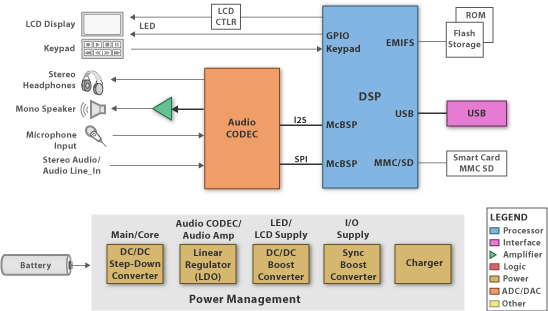
\epsfig{file=figures/Fig_3_4_DSP_MP3,width=0.9\textwidth}\\
	  \caption{MP3-Player, an Application for DSP-Processors}
     \end{center}
\end{figure}
\os{\newpage}

\item[{\rot\bf Microcontrollers for Embedded Systems }]~\\[-3ex]
\os{\bigskip}
\bi
	\ite most embedded systems employ a microcontroller
	\ite differences in the use of internal memory and/or external memory
	\ite human interface almost nonexistent or really small
	\bigskip 
	\ite according to the reduction of hardware costs more functions imlemented in a processor
	\ite a combination of microcontroller and signal processor are build (OMAP-Processor, part of the Beagle-Board)
	
\ei
\os{\newpage}

\begin{figure}[!hbtp]
     \begin{center}
	  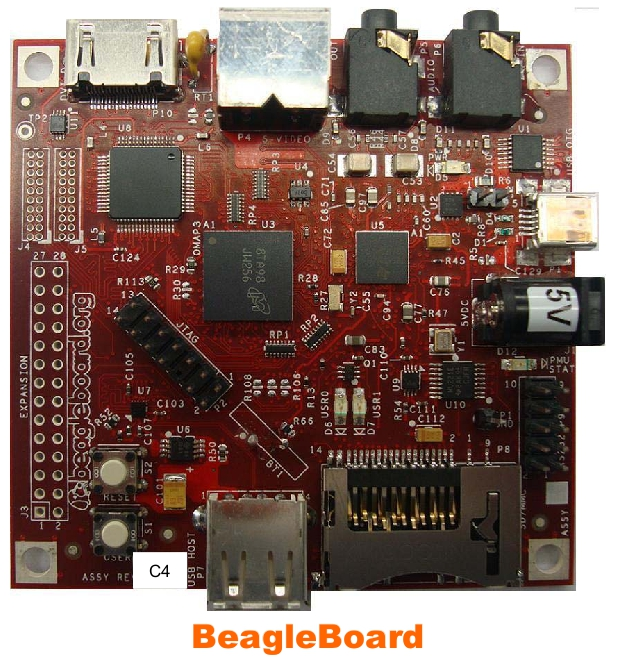
\epsfig{file=figures/Fig_3_5_BeagleBoard,width=0.5\textwidth}\\
	  \caption{Beagle Board with OMAP-Processor}
     \end{center}
\end{figure}
\os{\newpage}     

\item[{\rot\bf Components of the microcontroller/signal processor based Beagle Board }]~\\[-3ex]
\os{\bigskip}
\bi
	\ite microcontroller ARM Cortex-A8 (wordlength 32 Bit)
	\ite signalprocessor TMS 320DM641 (fix point digital signal processor, wordlenth 32 bit, multi media control and interfaces) 
	\ite TPS 65950 Reset and Power Management
	\ite TFP 410 Interface to external LCD panels
	\ite different digital interfaces (I/0)
	
\ei
\os{\newpage}

\begin{figure}[!hbtp]
     \begin{center}
	  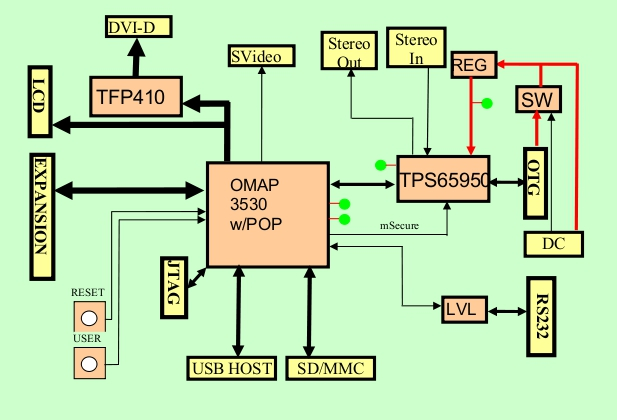
\epsfig{file=figures/Fig_3_6_ProcessorsBeagleBoard,width=0.8\textwidth}\\
	  \caption{Blockdiagram of a Beagle Board with different Processors}
     \end{center}
\end{figure}
\os{\newpage}

\begin{figure}[!hbtp]
     \begin{center}
	  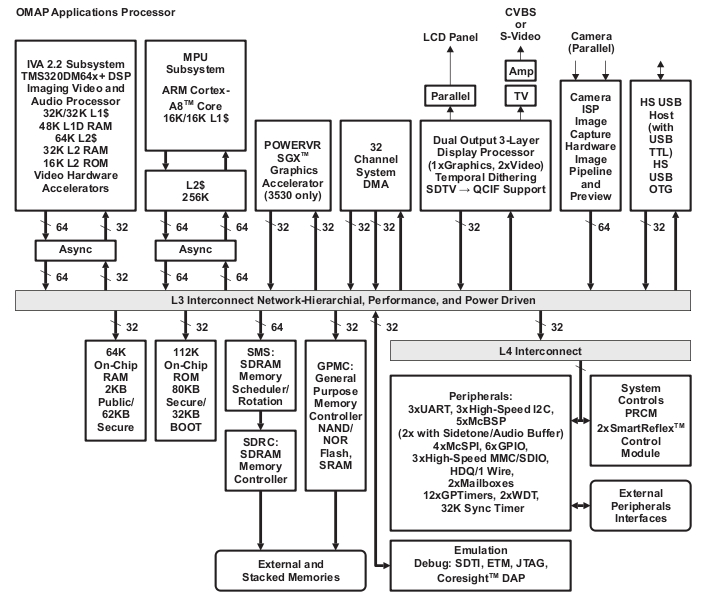
\epsfig{file=figures/Fig_3_7_InternalOMAP,width=0.7\textwidth}\\
	  \caption{Features of a OMAP-Processor}
     \end{center}
\end{figure}
\os{\newpage}     
\end{description}

%%%%%%%%%%%%%%%%%%%%%%%%%%%%%%%%%%%%%%%%%%%%%%%%%%%%%%%%%%%%%%%%%%%%%%%%%%%
\section{Overview about ARM Processors}
%%%%%%%%%%%%%%%%%%%%%%%%%%%%%%%%%%%%%%%%%%%%%%%%%%%%%%%%%%%%%%%%%%%%%%%%%%%
\begin{description}
\bigskip
\item[{\rot\bf Background }]~\\[-3ex]
\bi
	\ite ARM-Processors mostly part of a SoC (System on chip)
	\ite ARM-Processor itself is a IP-Core (intellectual property core), means a lisenced part which contains the processor funtionality
	\ite ARM-IP-Cores placed in a lot of different boards (like smart phones, embedded systems) and in the beagle bord  
	\bi 
		\ite same register model for address- and data register.
		\ite implementation of a 'load/store' architecture
		\ite use super user- and a user mode. (Priority of execution)
	\ei
	\ite implementation of superscalar architecture (Processing unit focused on integer processing).
	\ite integration of FPU coprocessor (NEON Processing unit focused on Floating Point processing). 
	\ite in some processors a MMU (\underline{m}emory \underline{m}anagement \underline{u}nit) is implemented (important for operation systems)
	\ite supports SIMD-applications.
	\ite integration of a lot of interfaces 
\ei

\os{\newpage}

\begin{figure}[!hbtp]
     \begin{center}
	  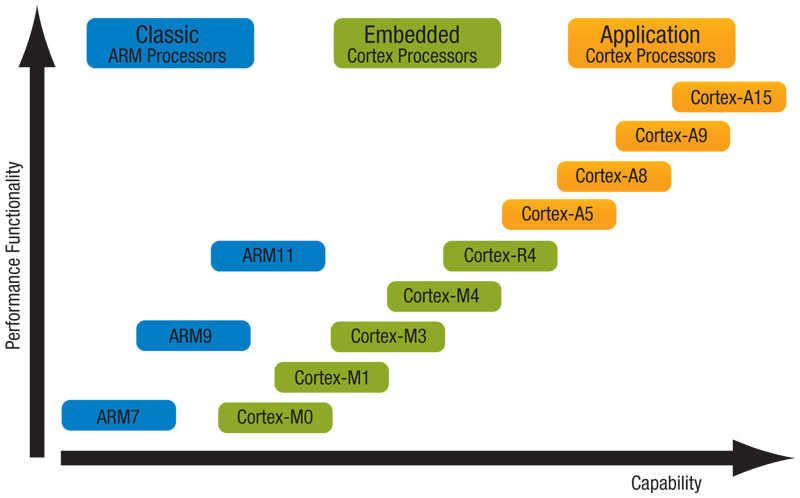
\epsfig{file=figures/Fig_3_8_ARMProcessors,width=0.85\textwidth}\\
	  \caption{Overview about different ARM-Processors}
     \end{center}
\end{figure}
\os{\newpage}
\end{description}



%%%%%%%%%%%%%%%%%%%%%%%%%%%%%%%%%%%%%%%%%%%%%%%%%%%%%%%%%%%%%%%%%%%%%%%%%%%
\section{Functions of the ARM-Cortex-A8-Processor}
%%%%%%%%%%%%%%%%%%%%%%%%%%%%%%%%%%%%%%%%%%%%%%%%%%%%%%%%%%%%%%%%%%%%%%%%%%%
\begin{description}
\item[{\rot\bf General Functions }]~\\[-3ex]
\bigskip
\bi
	\ite ARM-architecture is a RISC-architecture (\underline{r}educed \underline{i}nstruction \underline{s}et \underline{c}omputer)
	\ite according to the RISC-architecture more register banks are available (for every processor unit)
	\ite wordlength of the integer unit (and address unit) 32 Bit (wordlength of general purpose register 32 bit)
	\ite implements a superscalar architecture 
	\ite internal Harvard architecture based on two different caches- Instruction and Data (I-Cache and D-Cache respectively).
	\ite memory management unit (MMU).
	\ite different instruction set for: 
	\bi 
		\ite Thumb-instruction set (16 bit integer unit)
		\ite ARM-instruction set (32 bit integer unit)
		\ite ThumbEE-instruction set (32 bit integer unit without MMU)
		\ite NEON-, VFP-instruction set (for SIMD applications in integer (NEON) or floating point format (VFP)
		\ite FP-instruction set (for single floating point numbers) 
	\ei
\ei

\os{\newpage}
\begin{figure}[!hbtp]
     \begin{center}
	  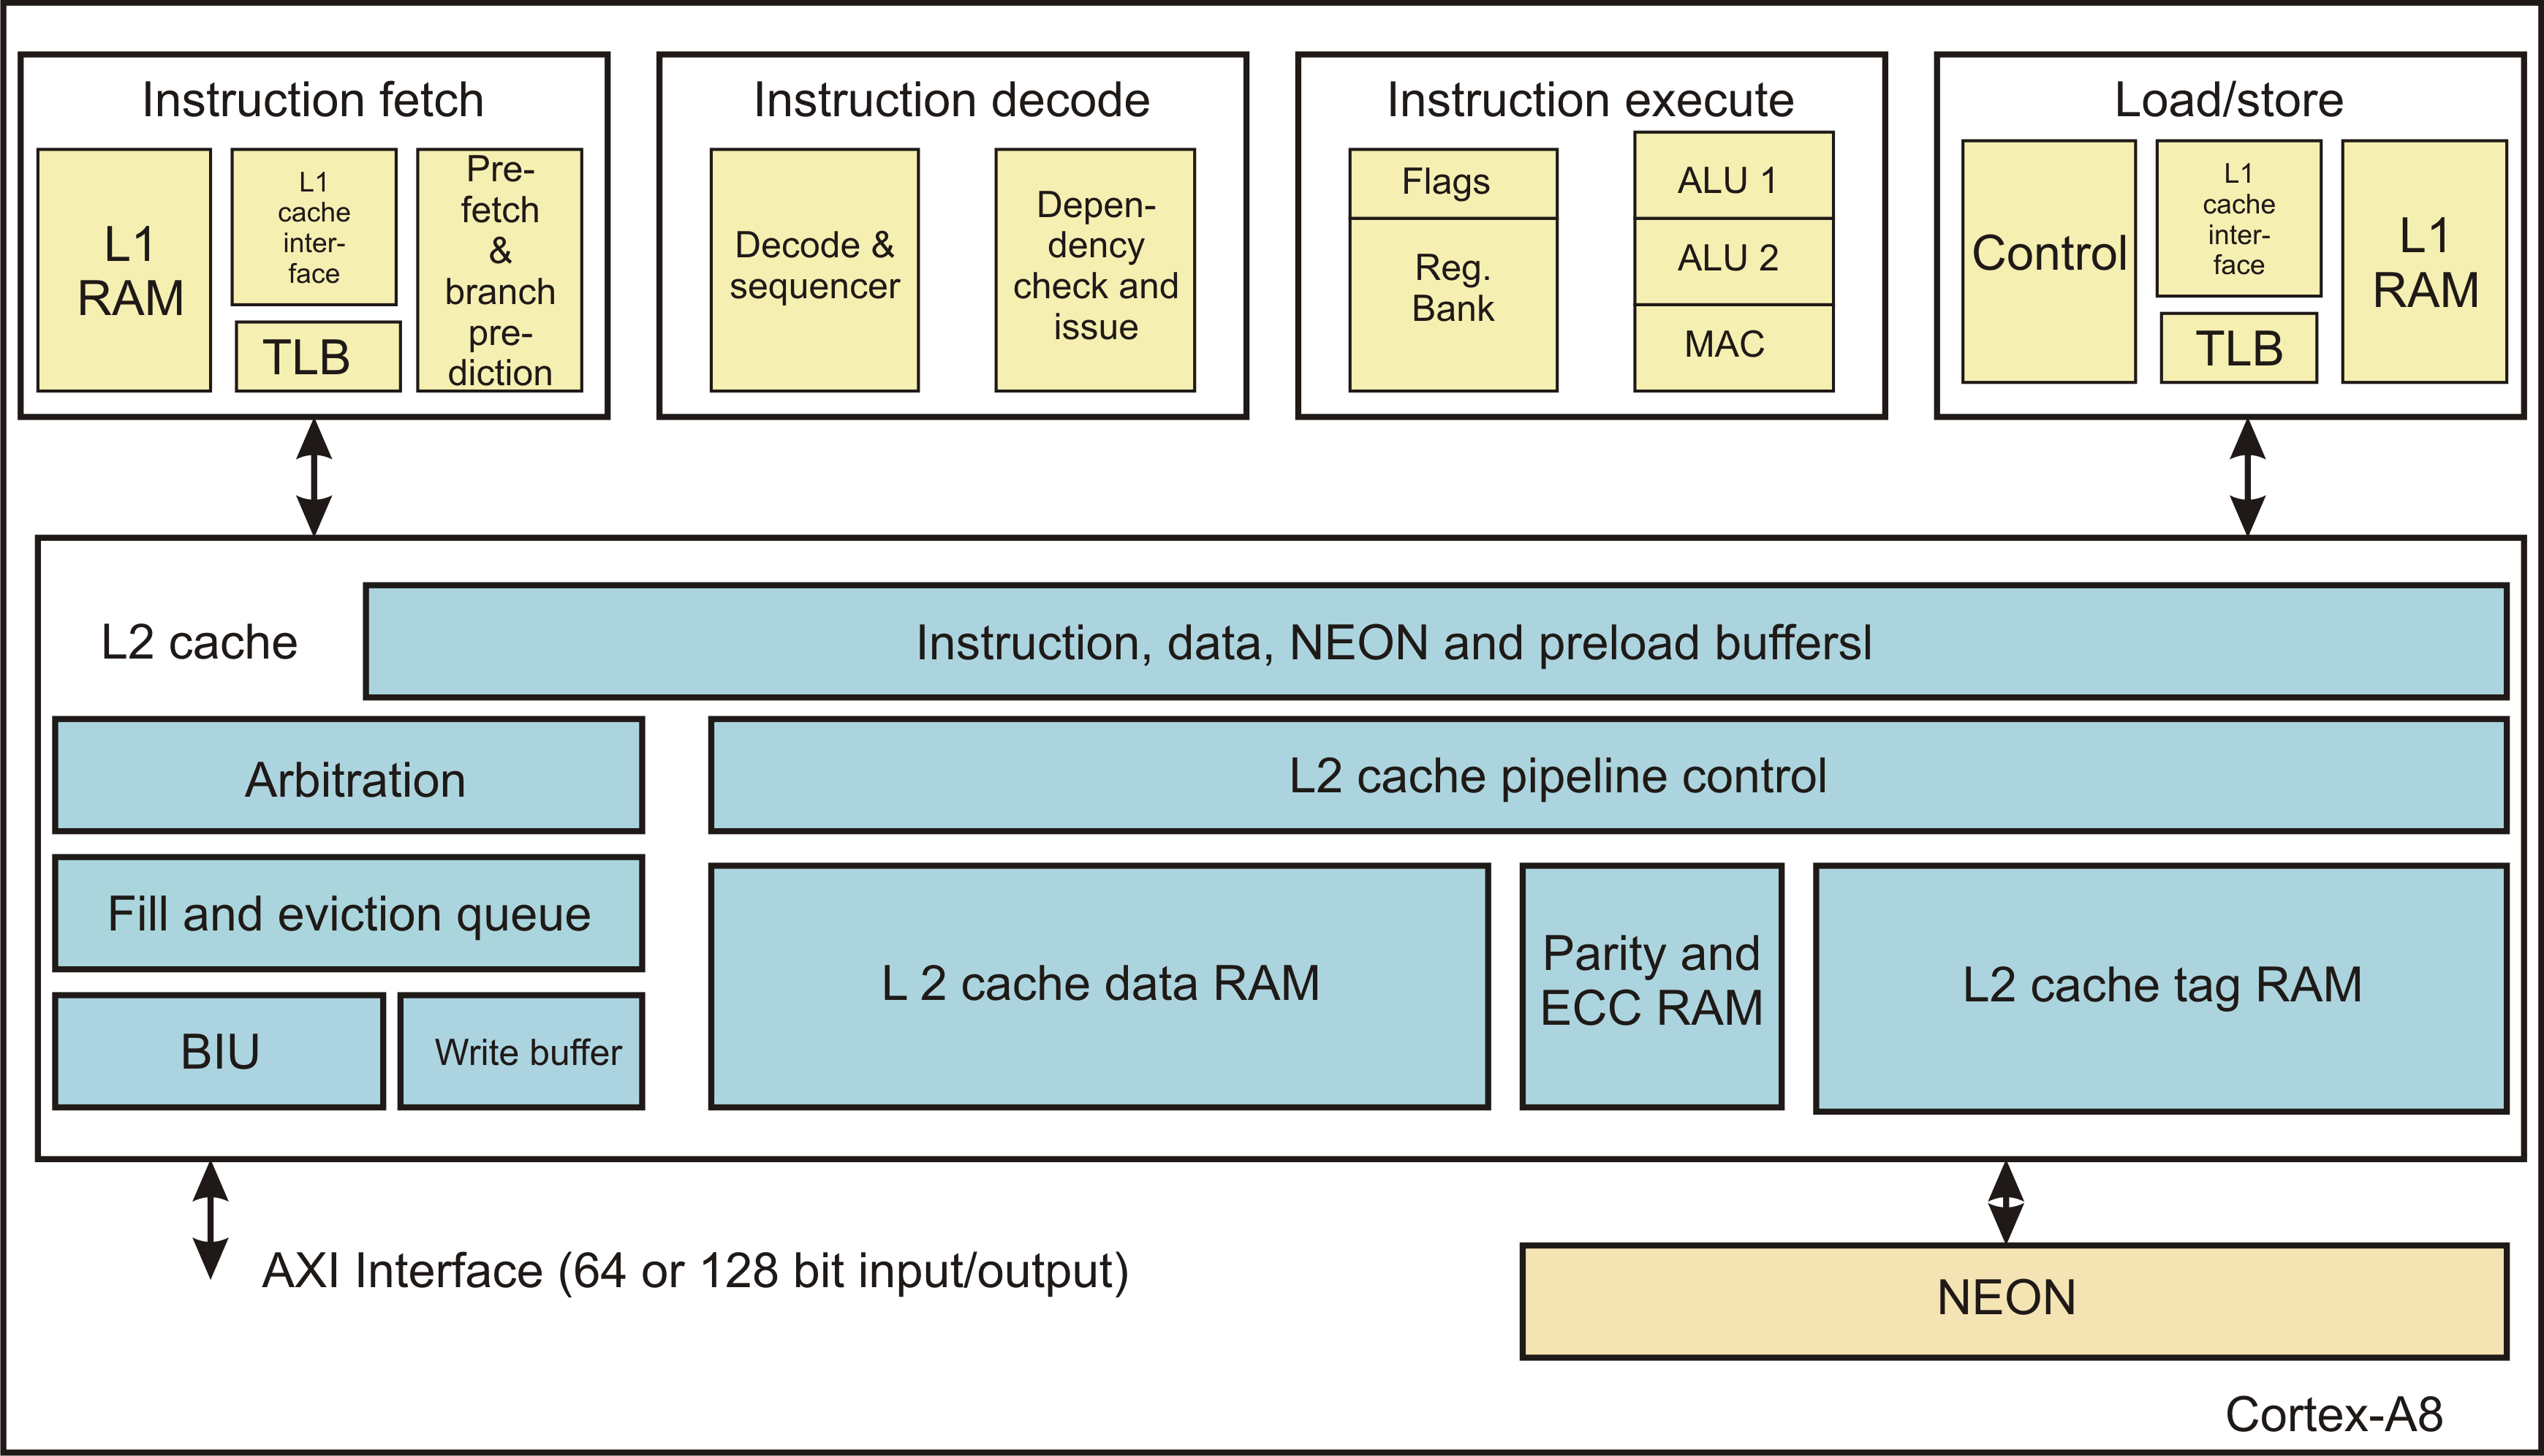
\epsfig{file=figures/Fig_3_9_Cortex.png,width=0.95\textwidth}\\
	  \caption{Blockdiagram Cortex-A8-Processor}
     \end{center}
\end{figure}     
\os{\newpage}

\item[{\rot\bf ALU1,2 }]~\\[-3ex]

\bi 
	\ite both ALU (ALU1 and ALU2) contains 32-bit integer units (could be used for signed, unsigned and fix point operations).
	\ite standard wordlength 32 bit
	\bi 
		\ite word 32 bit (data manipulation, address operations)
		\ite halfword 16 bit (data) 
		\ite byte 8 bit (data)
		\bigskip
		\ite doubleword 64 bit (data)
	\ei
	\bigskip 
	\ite works with RISC-operation on fixed length instructions (32 bit).
	\bi
		\ite load/store technique used
		\ite in every instruction a register is involved (as a source or destination register)
		\ite the order of operands are allways the same 
		\ite special data transfer instruction implemented for a read access (load) and a write access (store)
		\ite function calls work register based (not memory based as for CISC-processors)
		\ite conditions could be used for transfer and data manipulation instructions
	\ei
	\ite pipeline not visible for the user (only in some special instructions an insert of NOPs are necessary to synchronize the pipeline).
	\ite to support the pipeline operation for branches (especially conditional branches) a branch cache is involved.
	\ite three different instruction sets are available for the ALU
	\bi
		\ite Thumb instruction set for 16 bit applications
		\ite ThumbEE instruction set for 32 bit applications (typical embedded applications)
		\ite ARM instruction set for 32 bit application and the support of virtual memory management systems
	\ei
\ei
\os{\newpage}
\begin{figure}[!hbtp]
     \begin{center}
	  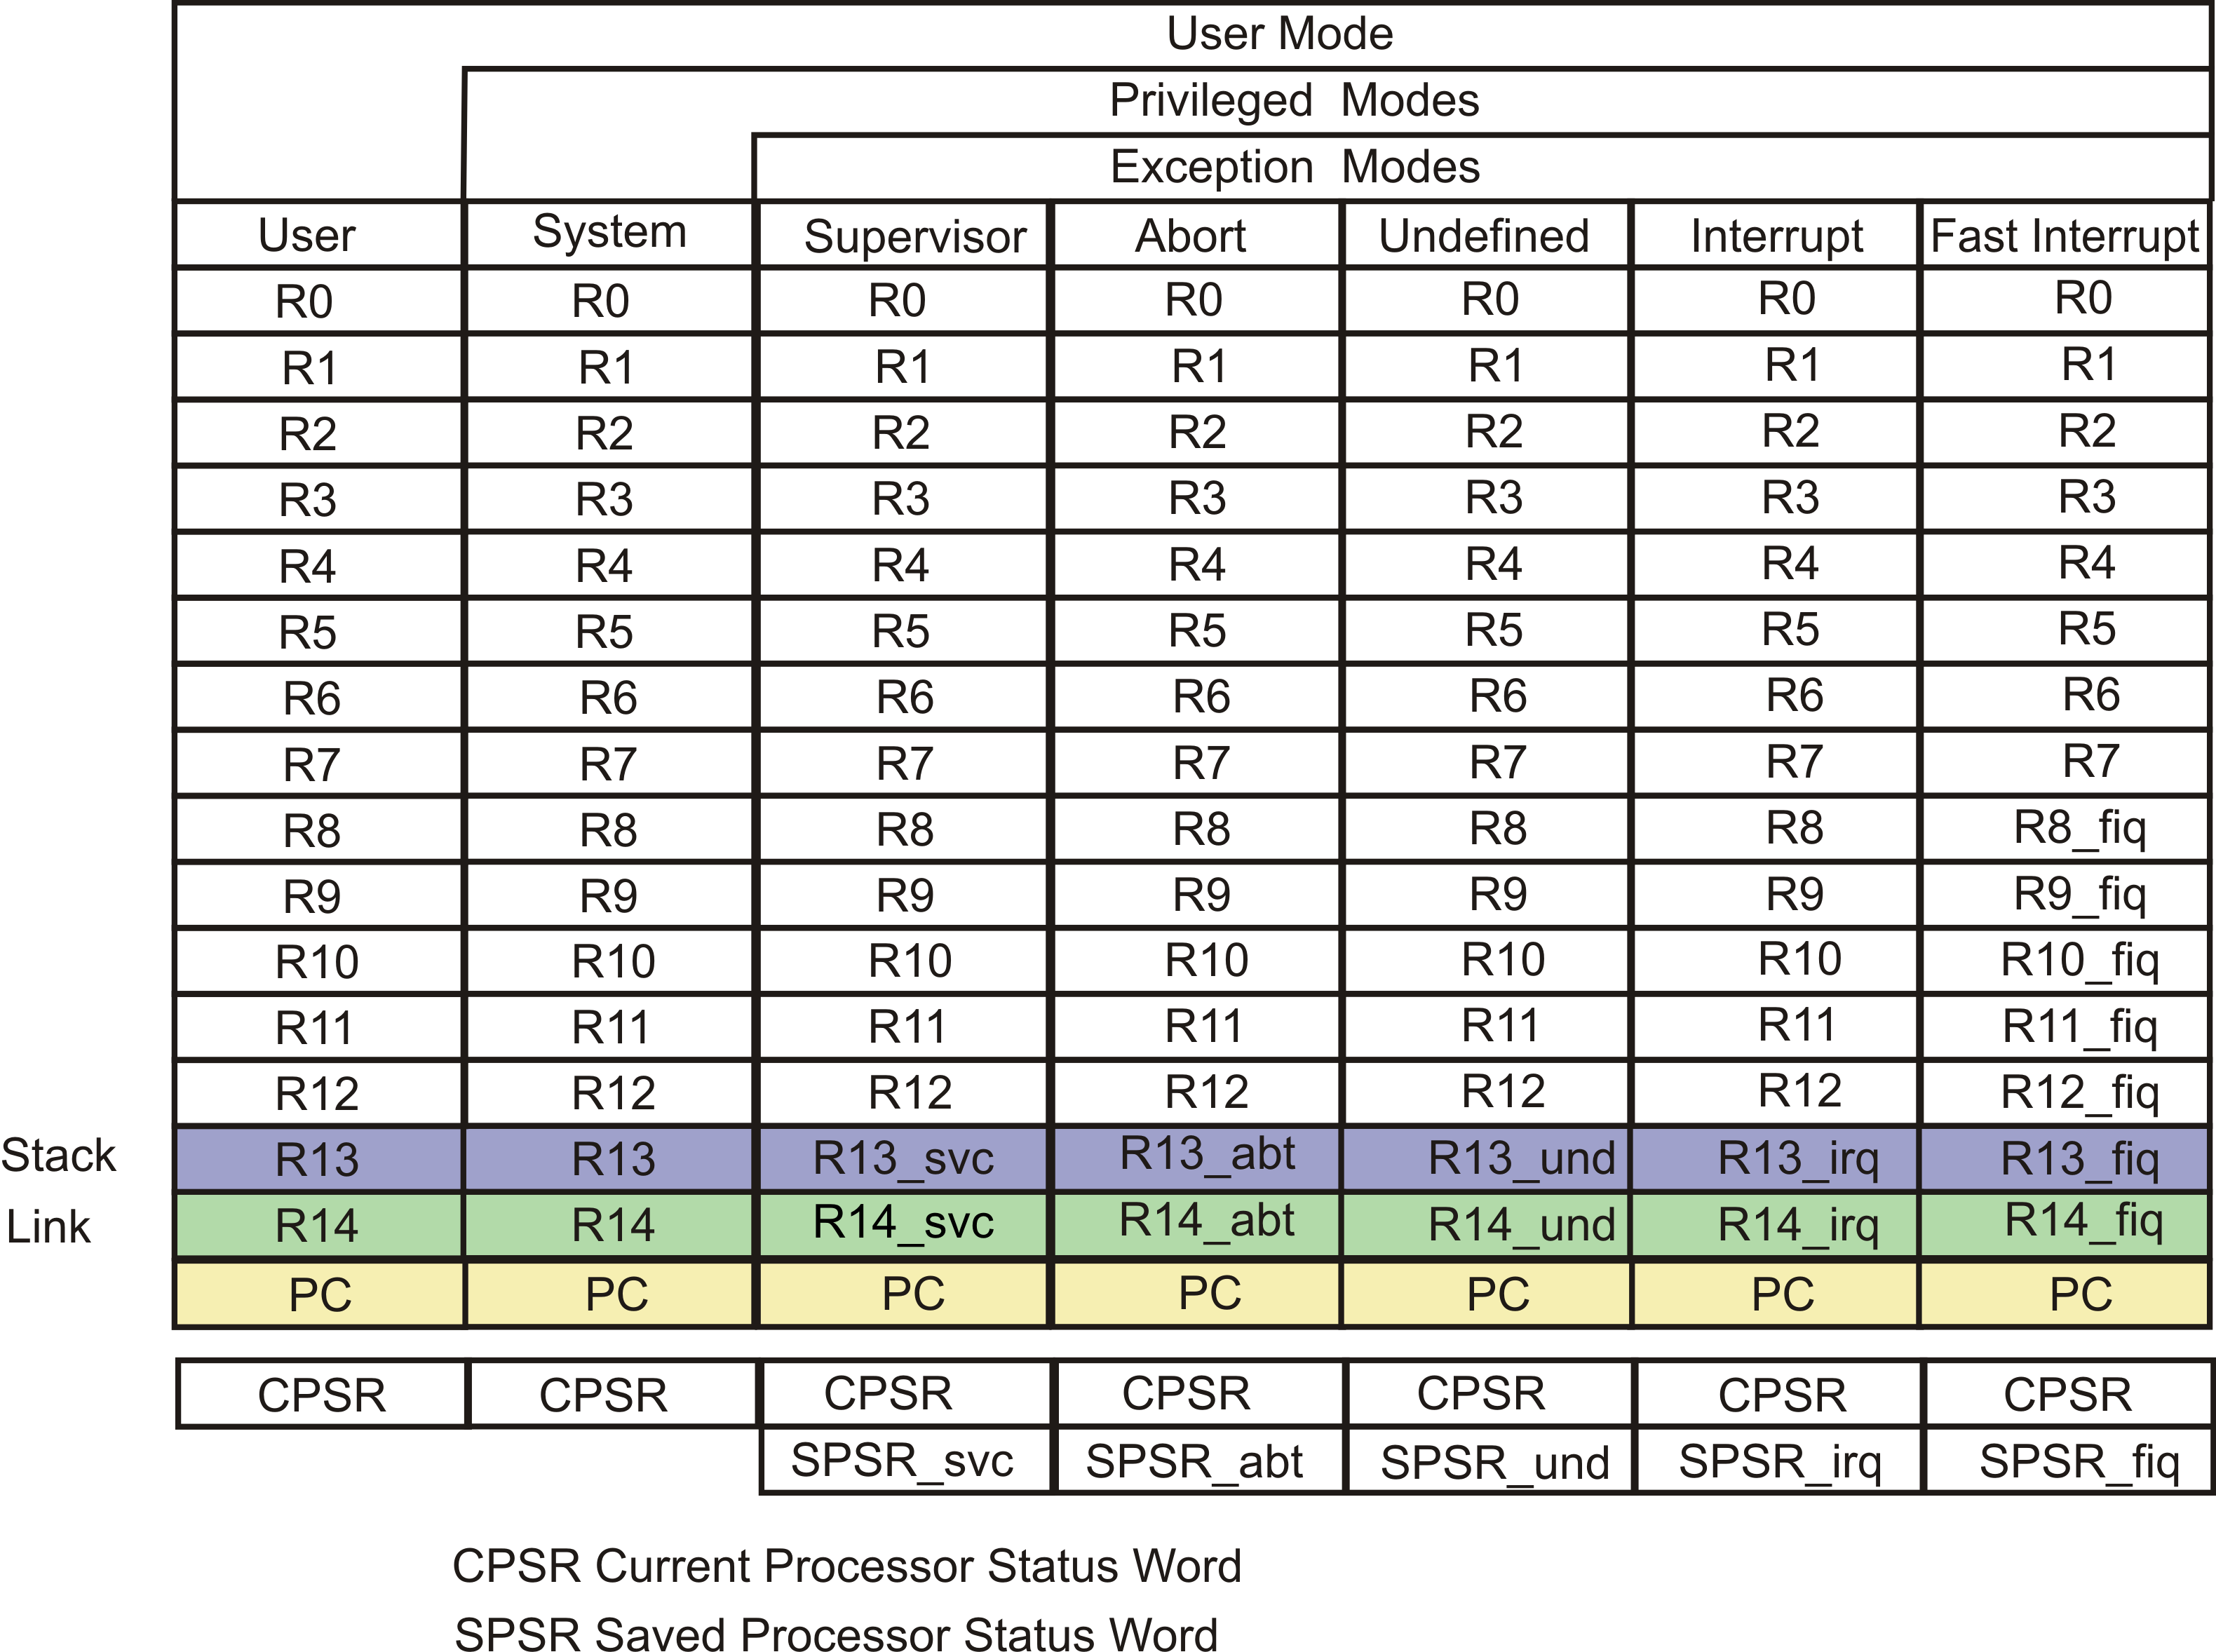
\epsfig{file=figures/Fig_3_10_RegisterSet.png,width=0.8\textwidth}\\
	  \caption{Register Set of the ALU}
     \end{center}
\end{figure}
\os{\newpage}

\bi
      \ite ALU (and the processor) runs in seven different modes
      \ite register set from r0 - r12 in every mode visible (without fast interrupt mode)
      \ite in exception modes the contains of the current processor status register (CPSR) are automatically saved (SPSR) (before the exception procedure starts) 
      \ite modes 
      \bi
		\ite user \pr standard mode
		\ite system \pr mode for operating systems
		\ite supervisor \pr mode for operating systems (mode after a reset)
		\ite abort \pr illegal instruction, illegal data operation
		\ite undefined \pr undefined instruction detected
		\ite interrupt \pr external interrupt
		\ite fast interrupt \pr internal interrupt (trap)
      \ei
\ei

\os{\newpage}
\item[{\rot\bf MAC (\underline{m}ultiply and \underline{ac}cumulate}]~\\[-3ex]

\bi 
	\ite part of the standard multiply function 
	\ite supports a multiplication and a add-operation in one instruction
	\ite different wordlength and signed/unsigned numbers are supported
	\ite typical examples (wordlength)
	\bi 
		\ite 32 = 32 +/- 16 x 16.
		\ite 32 = 32 + 16 x 16 + 16 x 16
		\ite 32 = 16 x 16
		\ite 64 = 64 +/- 32 x 32
		\ite 64 = 64 +/- 16 x 16
		\ite 64 = 32 x 32
	\ei
 
\ei
\os{\newpage}
\item[{\rot\bf NEON / VFP (SIMD and vector processing of integer and floating point numbers)}]~\\[-3ex]
\bi 
	\ite supports integer (fix point) and floating point packed calculations (NEON) of 32 bit numbers
	\ite vector floating point numbers with 32 bit or 64 bit are processed by the VFP-unit
	\ite every floating point number is:
	\bi
		\ite normalized
		\ite there exists no carry bit or a doubling of the word format after a multiplication (very useful in combined arithmetical expressions)
		\ite every floating point number could be characterized (zero, normalized, denormalized, exist, free) 
	\ei
	\bigskip
	\ite operations on NEON- and VFP-unit works as
	\bi
		\ite scalar operation on single (s = 32 bit), double (d = 64 bit) or quad q = 128 bit) precision, the involved registers have not be placed at the beginning of a bank
		\ite vector operations on 4 single precision elements, the involved registers starts at the beginning ore in the middle of a bank
		\ite vector operations on 2 double precision elements, in this case the registers starts at the beginning ore in the middle of a bank
		\ite scalar operation on 1 quad precision element
	\ei
\ei
\os{\newpage}
\begin{figure}[!hbtp]
     \begin{center}
	  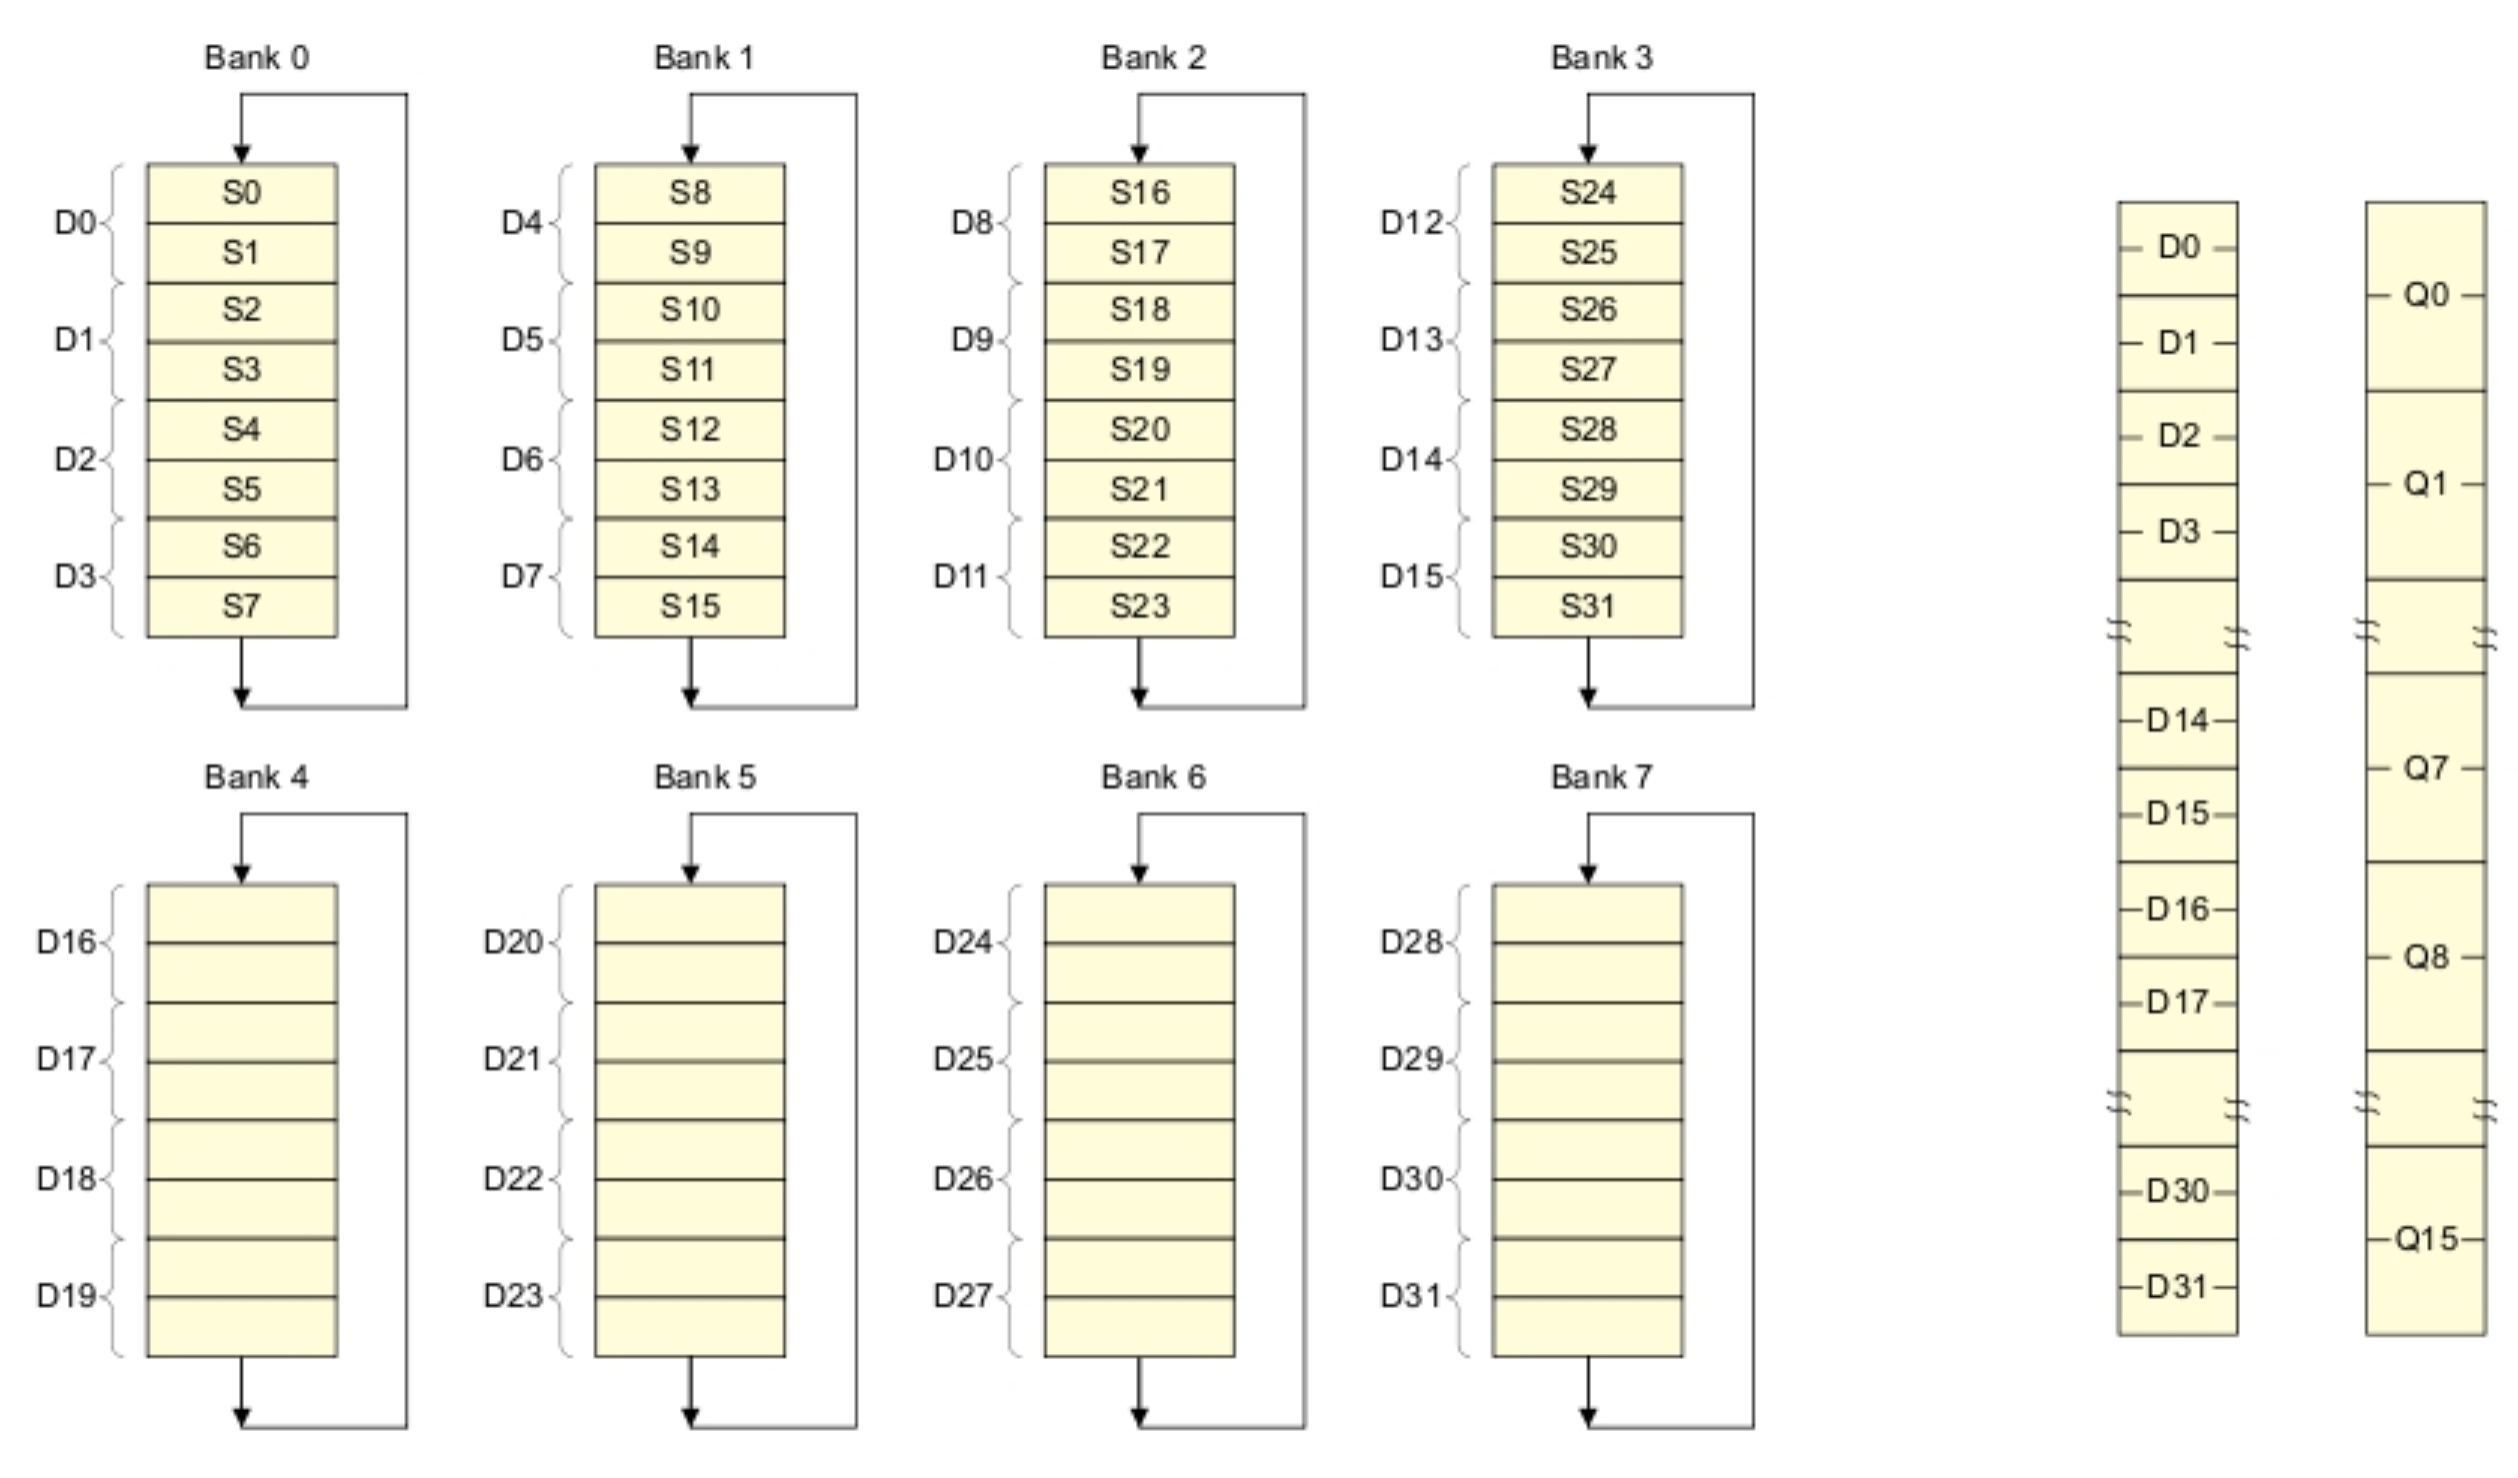
\epsfig{file=figures/Fig_3_11_NEON_VFP_Registers,width=0.9\textwidth}\\
	  \caption{Register set of NEON/VFP Coprocessor}
     \end{center}
\end{figure}
\os{\newpage}
 

\bi 
	\ite Examples for scalar and vector operations 
	\bi
		\ite scalar operation
		\ite FADDS S12, S21, S22
	\ei
	\bigskip
	\bi 
		\ite vector operation on single presision with 4 iterations
		\ite  FMACS S16, S0, S8 (instruction)
		\bigskip
		\\ FMACS S16, S0, S8  ; 1st iteration
		\\ FMACS S17, S1, S9  ; 2nd iteration
		\\ FMACS S18, S2, S10 ; 3rd iteration
		\\ FMACS S19, S3, S11 ; 4rd and last iteration
	\ei
	\bi 
		\ite vector operation on double presision with 2 iterations
		\ite  FMULD D12, D8, D2 (instruction)
		\bigskip
		\\ FMULD D12, D8, D2 ; 1st iteration
		\\ FMULD D13, D9, D3 ; 2nd and last iteration

	\ei 
\ei

\os{\newpage}
\item[{\rot\bf MMU (\underline{m}emory \underline{m}anagement \underline{u}nit) }]~\\[-3ex]

\bi 
	\ite supports a flexible, software-defined virtual environment.
	\ite in the case of virtual memory, the MMU supports 4-, 8-Kbyte, 1-Mbyte or 16-Mbyte page sizes.
	\ite the pages addressed with separate, 32-entry, fully associative instruction and data TLBs (TLBs \underline{t}ranslation \underline{l}ookaside \underline{b}uffer).
	\bi 
		\ite the separation of instruction- and data-TLB allows a parallel access of both instructions and data (Harvard-architecture).
		\ite the TLB works as registers (faster than memory based entries) 
	\ei
	\ite the MMU itself is memory-mapped (control, status, and fault registers)
	\ite the access to the MMU starts with a control-register 
	\ite MMU supports programmable address space priorisation steps (ASID \underline{a}ddress \underline{s}pace \underline{id}entifier).
\ei
\os{\newpage}
\begin{figure}[!hbtp]
     \begin{center}
	  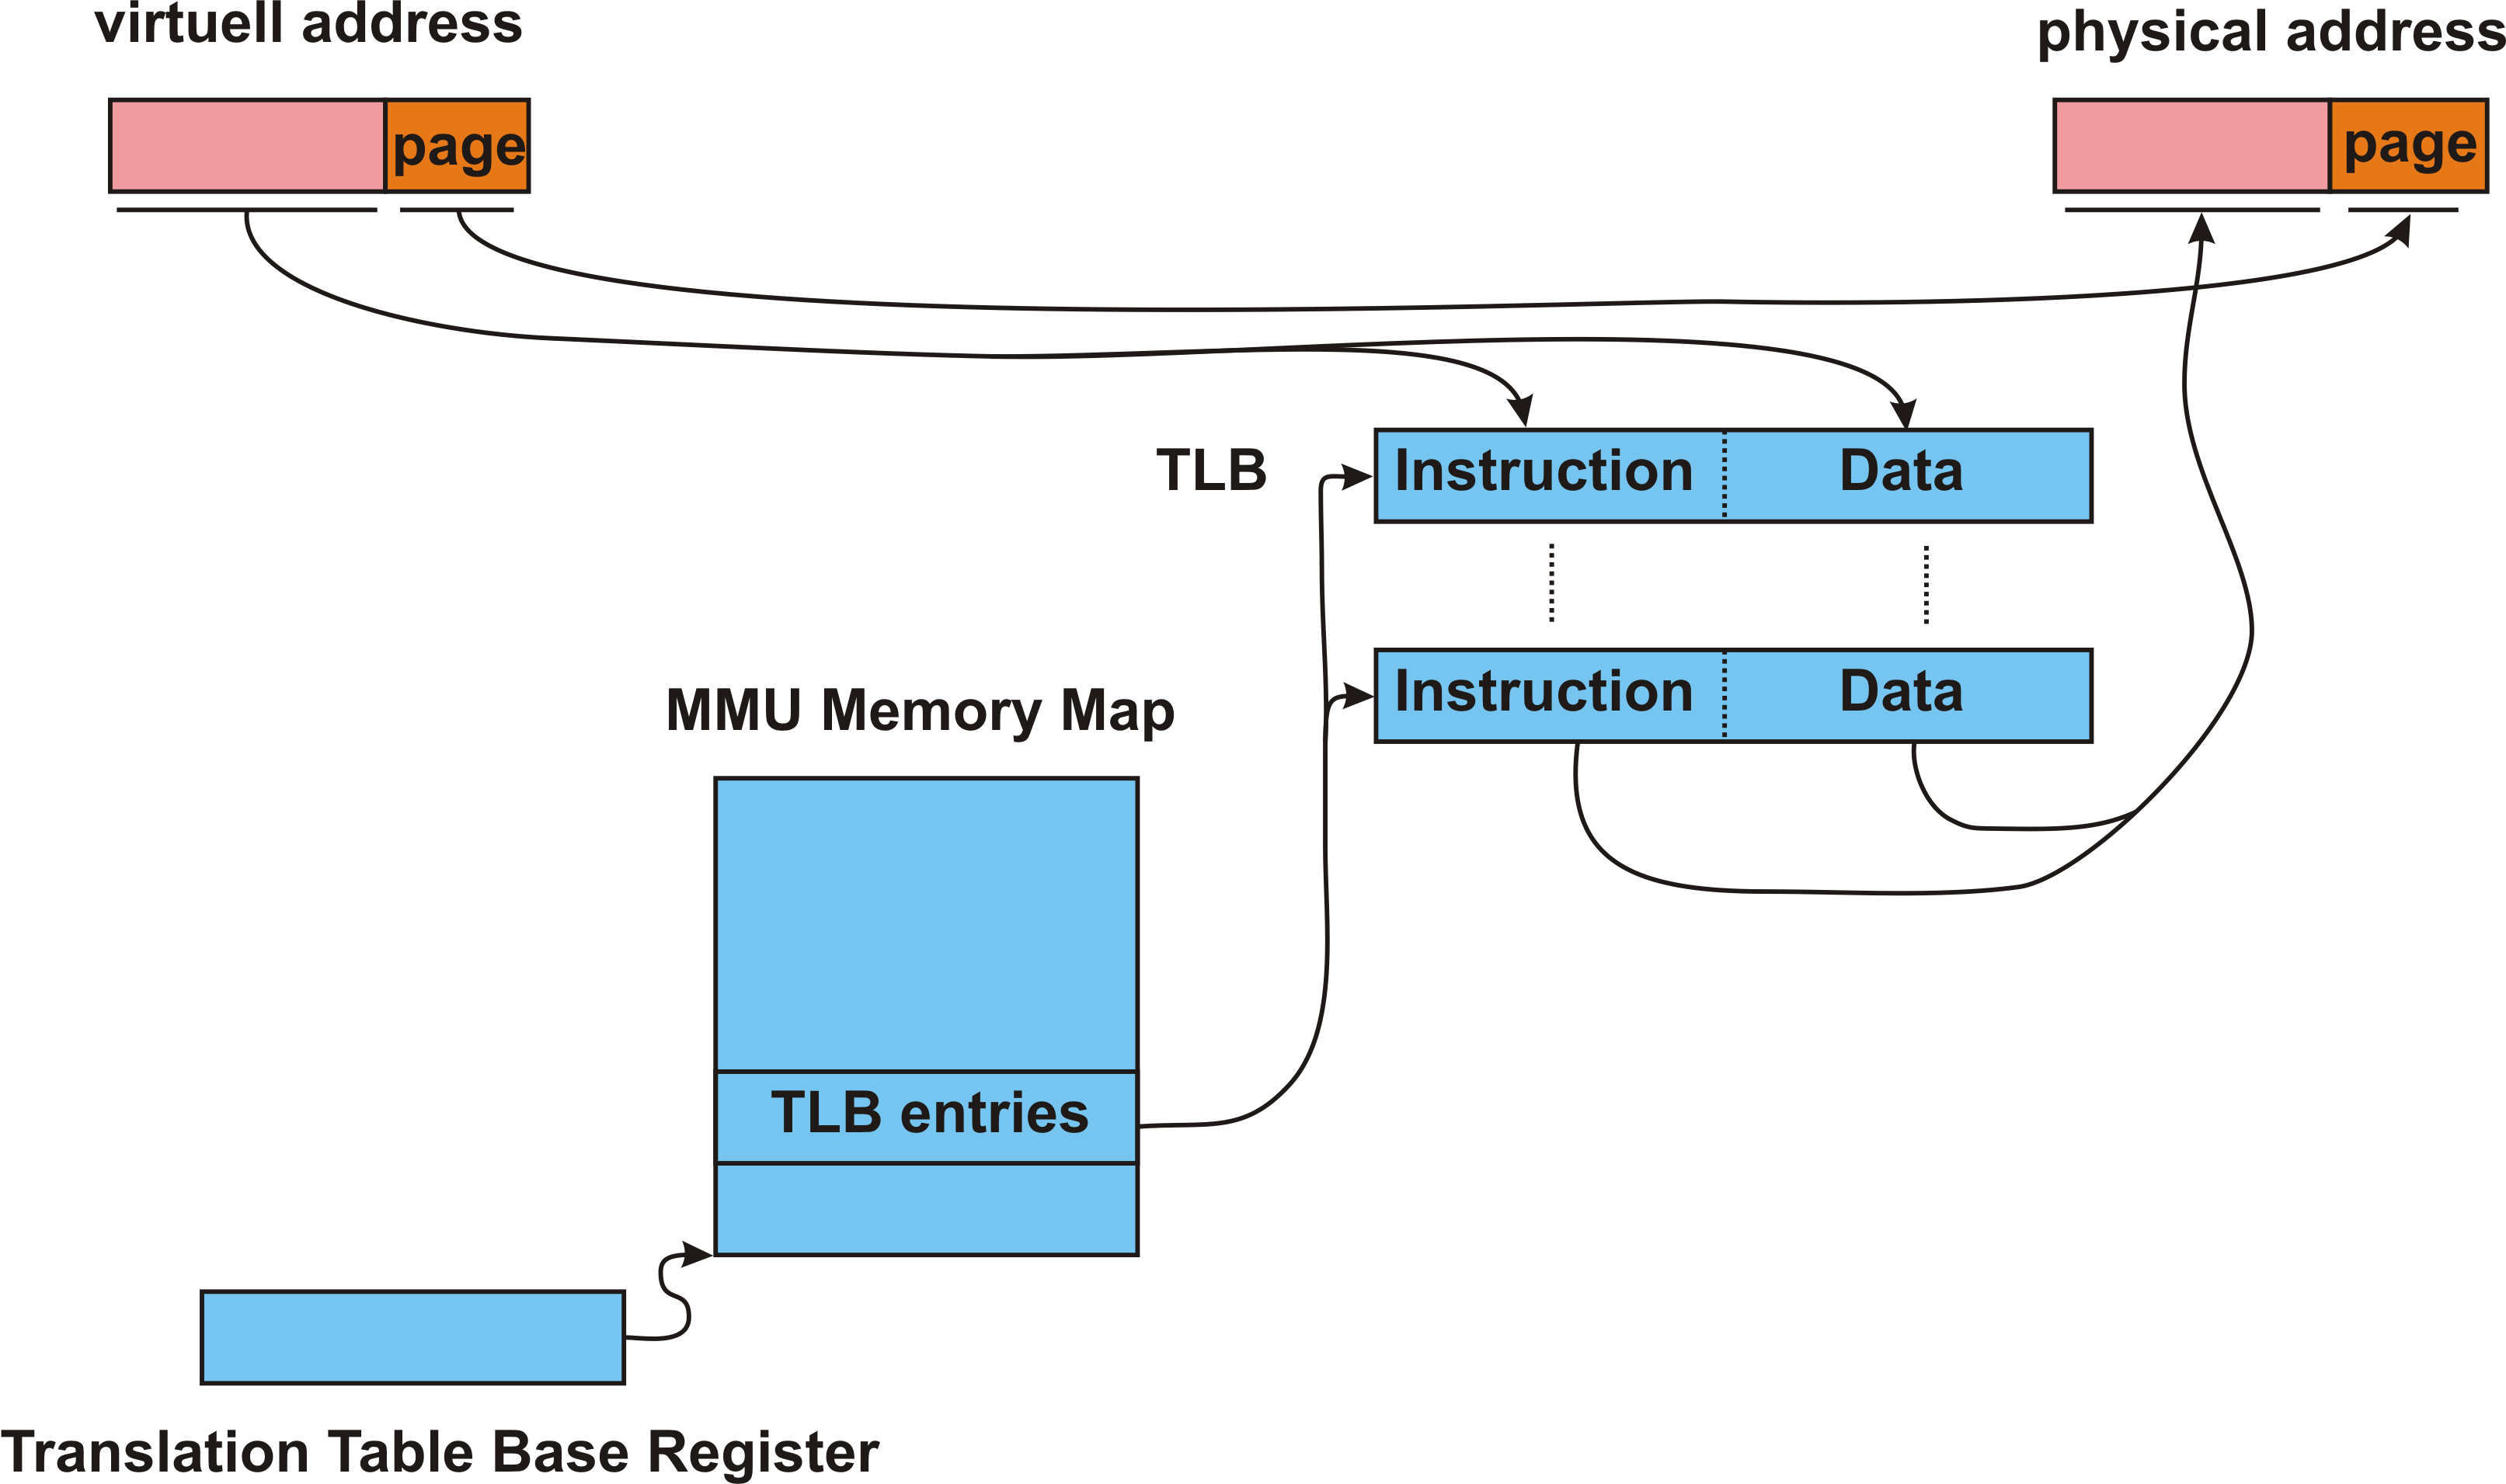
\epsfig{file=figures/Fig_3_12_MMU,width=0.8\textwidth}\\
	  \caption{Principal functions of the MMU}
     \end{center}
\end{figure}
\os{\newpage}

\begin{figure}[!hbtp]
     \begin{center}
	  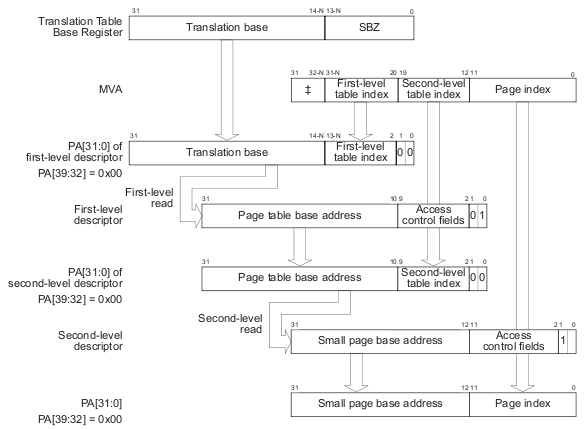
\epsfig{file=figures/Fig_3_13_Page_Address_Translation,width=0.8\textwidth}\\
	  \caption{Page Address Translation}
     \end{center}
\end{figure}
\os{\newpage}
\end{description}

%%%%%%%%%%%%%%%%%%%%%%%%%%%%%%%%%%%%%%%%%%%%%%%%%%%%%%%%%%%%%%%%%%%%%%%%%%%
\section{Overview about the DSP}
%%%%%%%%%%%%%%%%%%%%%%%%%%%%%%%%%%%%%%%%%%%%%%%%%%%%%%%%%%%%%%%%%%%%%%%%%%%
\begin{description}
\bigskip
\item[{\rot\bf DSP Functions and additional Features }]~\\[-3ex]
\bigskip
\bi
	\ite DSP supports the OMAP-Processors with   
	\bi 
		\ite processor funtionality to work on digital signal algorithm
		\ite internal RAM and ROM (data memory, Boot-ROM)
		\ite external RAM (SDRAM for instruction and data memory)
		\ite a lot of digital interfaces
	\ei
	\ite DSP is a 32 bit fix point processor
	 
\ei

\os{\newpage}
\begin{figure}[!hbtp]
     \begin{center}
	  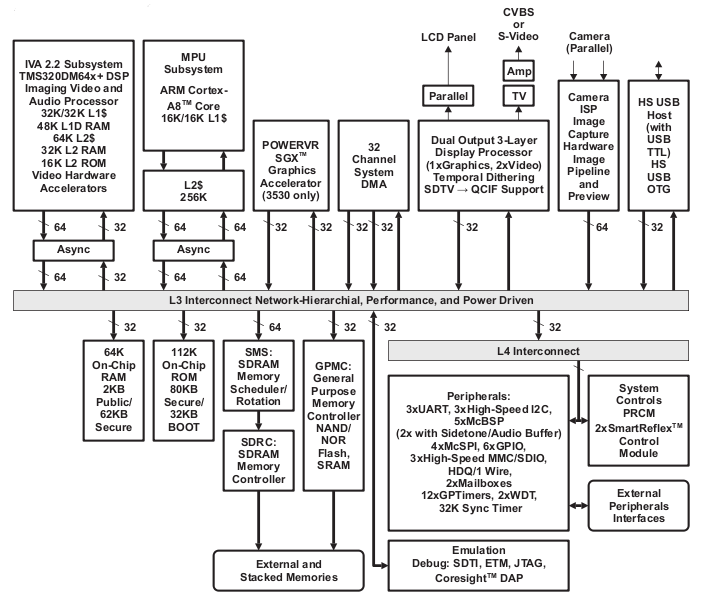
\epsfig{file=figures/Fig_3_14_OMAP_Blockdiagram,width=0.7\textwidth}\\
	  \caption{Overview about the Units in a OMAP-Processors}
     \end{center}
\end{figure}
\os{\newpage}

\item[{\rot\bf DSP (\underline{d}igital \underline{s}ignal \underline{p}rocessing) }]~\\[-3ex]
\bigskip
\bi
	\ite DSP processor with 64 x 32 bit registers grouped in two banks (bank A and bank B)
	\ite multiply add operational unit (MAC) (with a internal wordlength of 40 bits)
	\ite barrel shifter to scale the result
	\ite use internal memories (on the DSP-chip) to store up to 3 operands in 1 cycle
	\ite MAC-operation and barrel shifting-operation execute in 1 cycle
	\ite different interfaces for
	\bi 
		\ite connection to an external SDRAM
		\ite L2 cache system to coordinate parallel data transfers (for the transfer of both values in a multiplikation instruction)
		\ite internal timers
		\ite interrupt sources
	\ei
	\ite DSP is a VLIW-processor (\underline{v}ery \underline{l}ong \underline{i}nstruction \underline{w}ord)
	\bi
		\ite wordlength 256 bit
		\ite more instructions are placed in one instruction word (e.g. 2 transfers 4 arithmetical instructions)
		\ite one VLIW-instruction are excuted in one cycle
	\ei
\ei
\os{\newpage}
\begin{figure}[!hbtp]
     \begin{center}
	  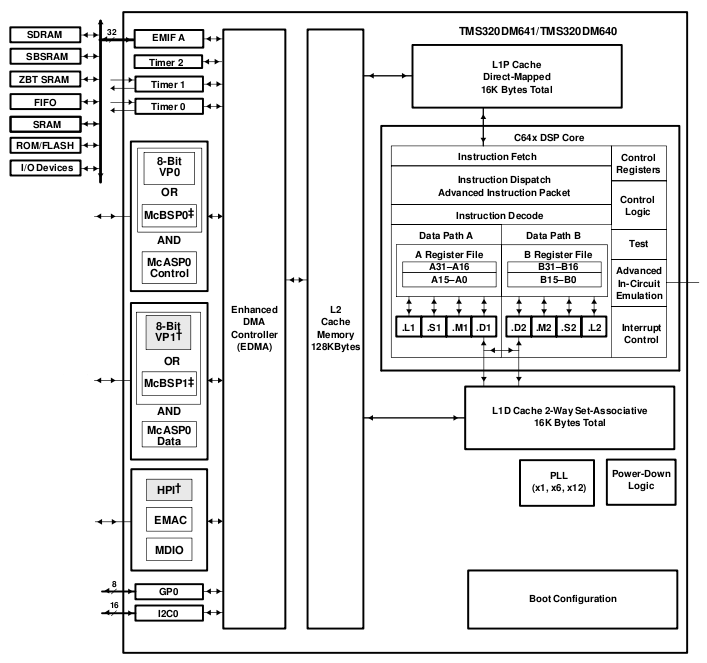
\epsfig{file=figures/Fig_3_15_Blockdiagram_TMS320DM641,width=0.6\textwidth}\\
	  \caption{Blockdiagram of the DSP-Part of the OMAP-Processor}
     \end{center}
\end{figure}
\os{\newpage}

\item[{\rot\bf I/O-Units }]~\\[-3ex]
\bigskip

\bi
      \ite additional to the processor (ARM-Cortex-A8) and the signal processor (DSP) many digital I/O-units implemented
      \ite all units are connected by two interprocessor busses (L3 and L4)
      \ite the communication are controlled by specific cache controllers and the according cache memories
      \ite all processors (internal memories) and the registers or memories of the I/O-units and the external memory are visible in the Global Memory Map
\ei 
\os{\newpage}
\begin{figure}[!hbtp]
     \begin{center}
	  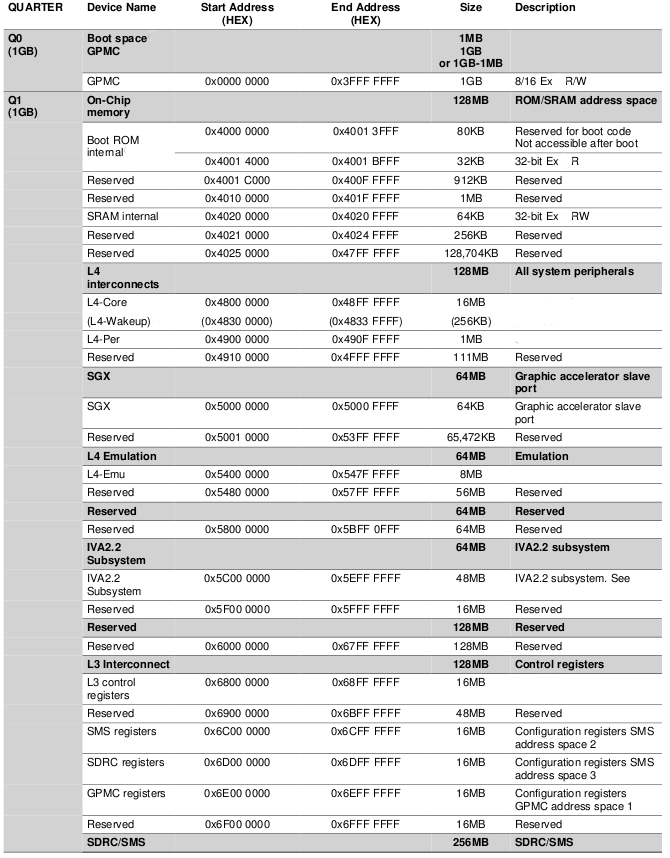
\epsfig{file=figures/Fig_3_16_MemoryMap_A,width=0.4\textwidth}\\
	  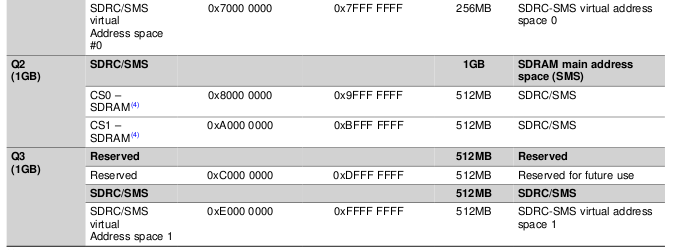
\epsfig{file =figures/Fig_3_16_MemoryMap_B,width=0.4\textwidth}\\
	  \caption{Global Memory Map of the OMAP-Processor}
     \end{center}
\end{figure}
\os{\newpage}

\bigskip
\bi
	\ite L3 interprocessor communication bus connects the processors and memory subsystems
	\ite L4 interprocessor communication bus connnects the processors with the I/O-systems
\ei
\os{\newpage}
\os{\bigskip}
\begin{figure}[!hbtp]
     \begin{center}
	  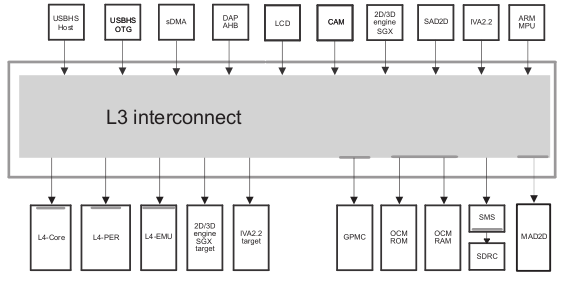
\epsfig{file=figures/Fig_3_17_L3_Interconnect,width=0.70\textwidth}\\
	  \caption{L3 Interprocessor Communication Bus}
     \end{center}
\end{figure}
\os{\newpage}

\begin{figure}[!hbtp]
     \begin{center}
	  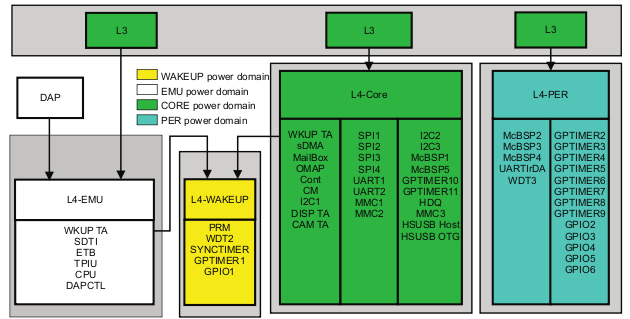
\epsfig{file=figures/Fig_3_18_L4_Interconnect,width=0.70\textwidth}\\
	  \caption{L4 Interprocessor Communication Bus}
     \end{center}
\end{figure}
\os{\newpage}

\bi
	\ite interprocessor communication and the communication between processors and the I/O-units are controlled by mailboxes
\ei

\os{\newpage}
\begin{figure}[!hbtp]
     \begin{center}
	  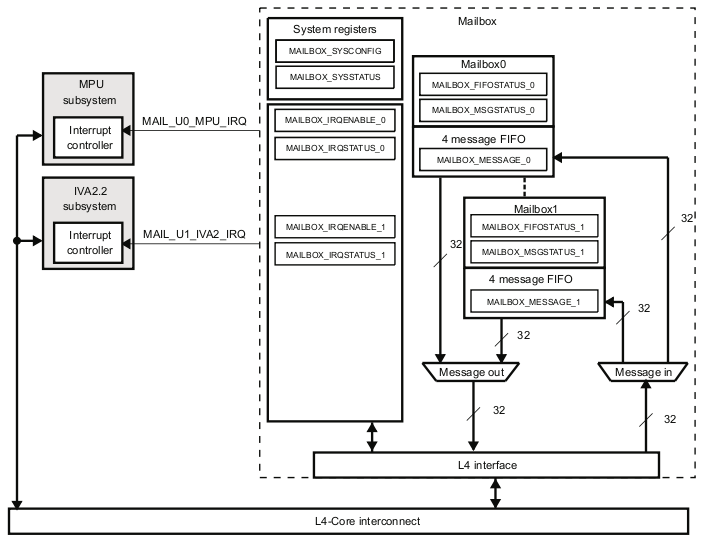
\epsfig{file=figures/Fig_3_19_Communication_Mailbox,width=0.70\textwidth}\\
	  \caption{Communication Mailbox}
     \end{center}
\end{figure}

\os{\newpage}
\begin{figure}[!hbtp]
     \begin{center}
	  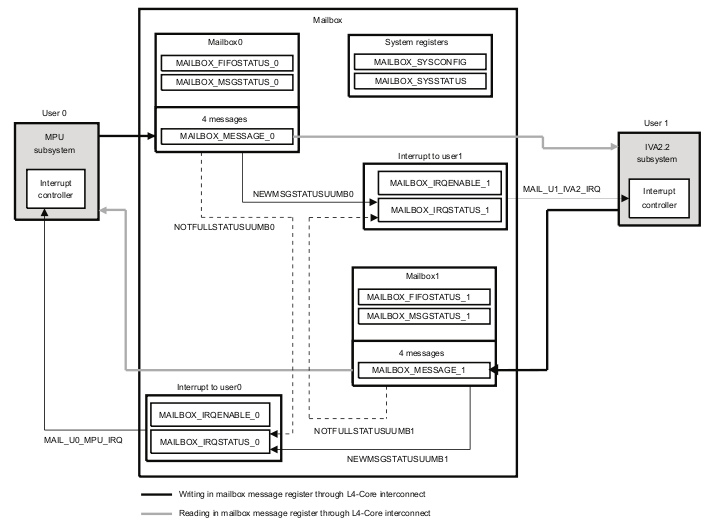
\epsfig{file=figures/Fig_3_20_Communication_Example,width=0.70\textwidth}\\
	  \caption{Example for Communications with Mailboxes}
     \end{center}
\end{figure}
\end{description}

